%%%
% Conférence « Comment bien démarrer son projet »
% Vendredi 03 décembre 2010
%%%

\section{Subversion}

\subsection{Généralités}
\begin{frame}{Pourquoi versionner~?}
  \begin{alertblock}{Concrètement}
    Les gestionnaires de versions vous permettent de~:
    \begin{itemize}
      \item gérer votre code source,
      \item conserver une trace toutes les modifications,
      \item revenir en arrière,
      \item travailler à plusieurs en partageant le code intelligement.
    \end{itemize}
  \end{alertblock}
  \begin{center}
    
\includegraphics[scale=3]{images/logo_svn} ~
    
\includegraphics[scale=0.7]{images/logo_git} ~
    
\includegraphics[scale=0.6]{images/logo_hg}
  \end{center}
  % Versionnement : permet de garder un trace de toutes les modifications
  % effectuées sur le code source. Possibilité de revenir en arrière,
  % travailler tous sur les même fichier sans conflit. Ajouter des
  % commentaires aux changements.
  % Il en existe plusieurs qui peuvent être assez différents les uns des
  % autres. On va s’intéresser à SVN car il est relativement simple et est
  % très répandu.
\end{frame}

\subsection{Utilisation typique}

\begin{frame}
  \texttt{checkout}
  \begin{center}
    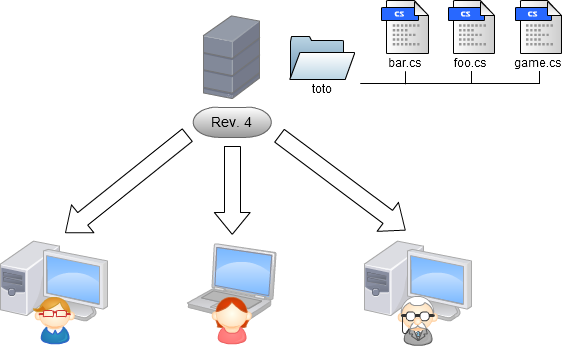
\includegraphics[scale=0.52]{images/1-CheckOut.png}
  \end{center}
	% Présentation du dépôt avec les trois fichier versionnés, du numéro de
	% révision. Checkout : récupère tout le contenu du dépot sous la dernière
	% version disponible.
\end{frame}

\begin{frame}
  \texttt{checkout}
  \begin{center}
    \vspace{-12pt}
    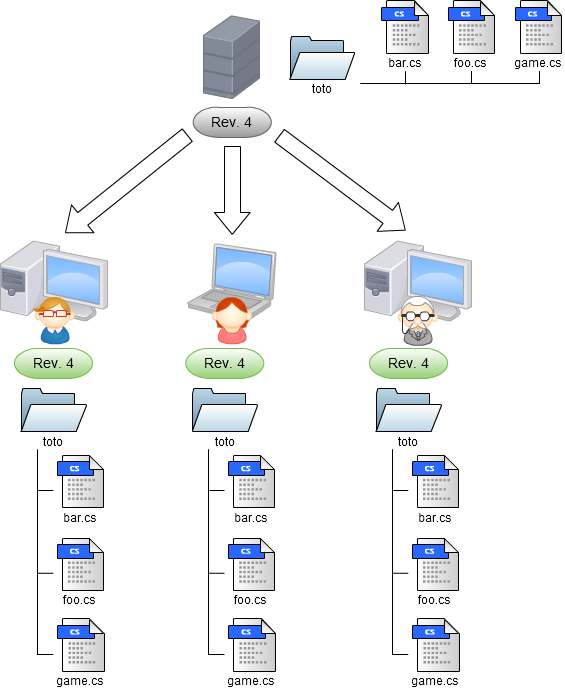
\includegraphics[scale=0.3]{images/2-CheckOut.png}
  \end{center}
	% Checkout fini : ils ont tous le contenu du dépôt, ils ont la dernière
	% version, révision 4.
\end{frame}

\begin{frame}
  \begin{center}
    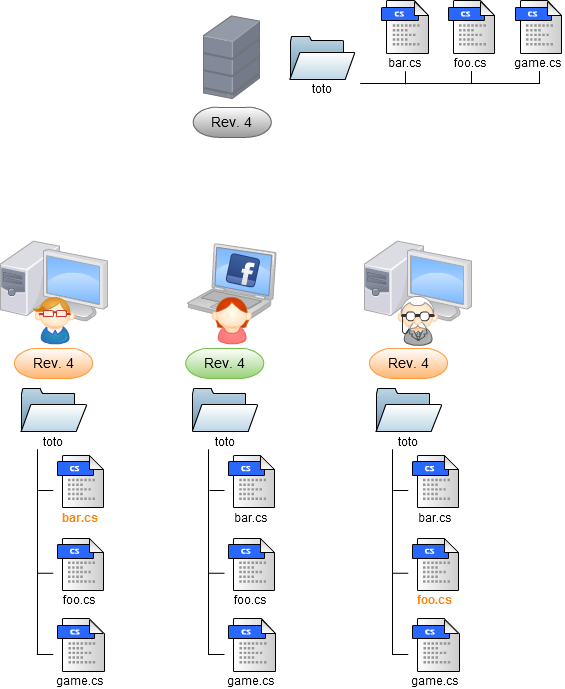
\includegraphics[scale=0.3]{images/3-Work.png}
	% Ils commencent à travailler sur les fichiers qui veulent. Il se sont
	% bien réparti les tâches : la femme et sur Facebook et les deux gars
	% travaillent chacun sur un fichier.
  \end{center}
\end{frame}

\begin{frame}
  \texttt{commit}
  \begin{center}
    \vspace{-12pt}
    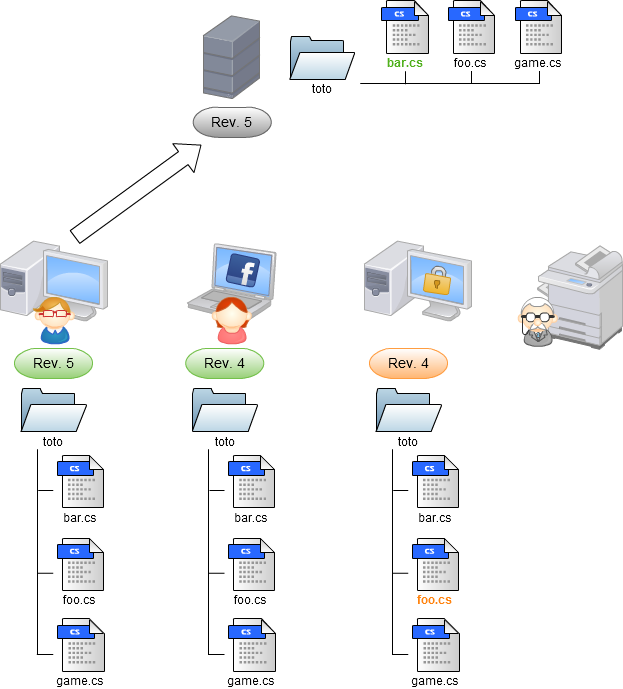
\includegraphics[scale=0.3]{images/4-Commit1.png}
  \end{center}
	% Quand le premier a fini son travaille, ça compile, ça marche, il va
	% commit : il va envoyer ses modifications sur le dépôt. Lui et le dépôt
	% passent en révision 5, les autres restent en révision 4. Les autres sont
	% occupés ailleurs.
\end{frame}

\begin{frame}
  \texttt{update}
  \begin{center}
    \vspace{-12pt}
    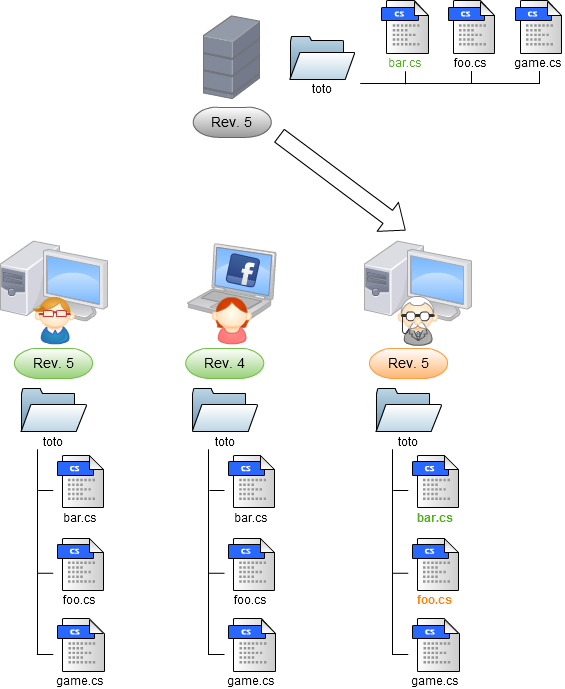
\includegraphics[scale=0.3]{images/5-Update.png}
  \end{center}
	% Le vieux revient et veux envoyer son travail. Mais avant de l’envoyer,
	% il fait un update : il récupère les modifications récentes depuis le
	% dépôt. Met à jour juste les fichiers modifiés sur le dépôt, ses
	% modifications locales ne changent pas.
\end{frame}

\begin{frame}
  \texttt{commit}
  \begin{center}
    \vspace{-12pt}
    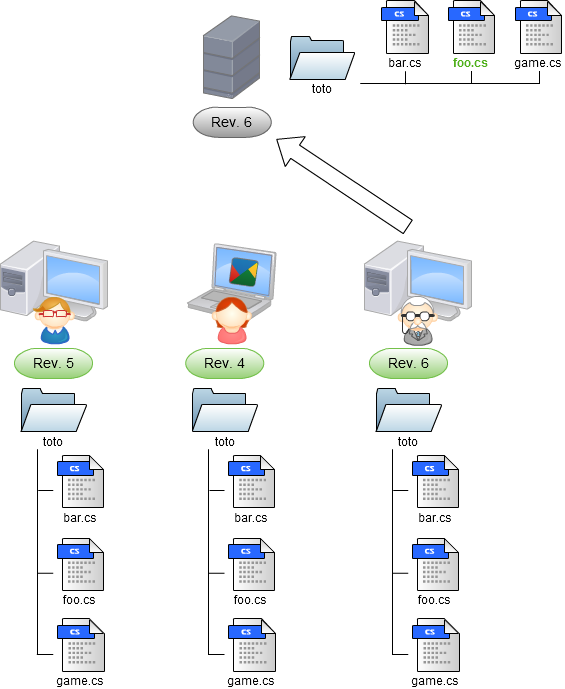
\includegraphics[scale=0.3]{images/6-Commit2.png}
  \end{center}
	% Le vieux envoie sont travail, le serveur passe en révision 6, le jeune
	% et la fille ne sont pas au courant.
	% La fille est passé sur Google Buzz.
\end{frame}

\begin{frame}
  \texttt{delete}
  \begin{center}
    \vspace{-12pt}
    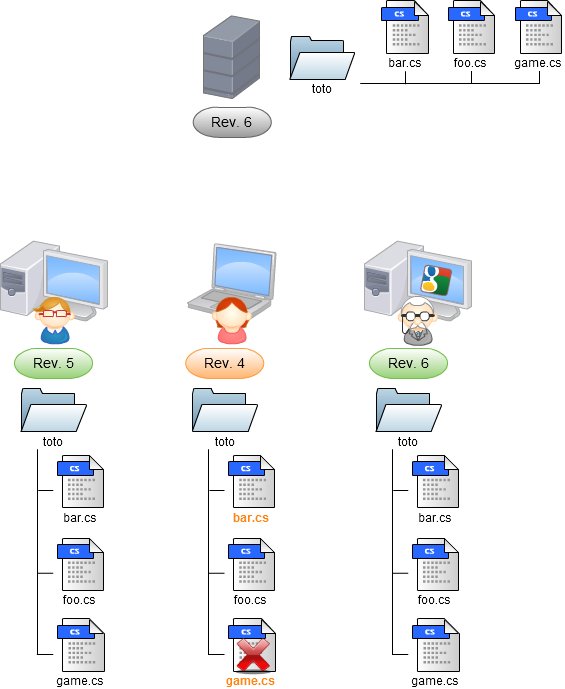
\includegraphics[scale=0.3]{images/7-Work.png}
  \end{center}
	% Elle décide de se mettre au travail et décide de supprimer game.cs par
	% ce que ça ne sert à rien selon elle.
	% Le vieux fait des recherches sérieuses sur Google pour le projet.
\end{frame}

\begin{frame}
  \texttt{commit}
  \begin{center}
    \vspace{-12pt}
    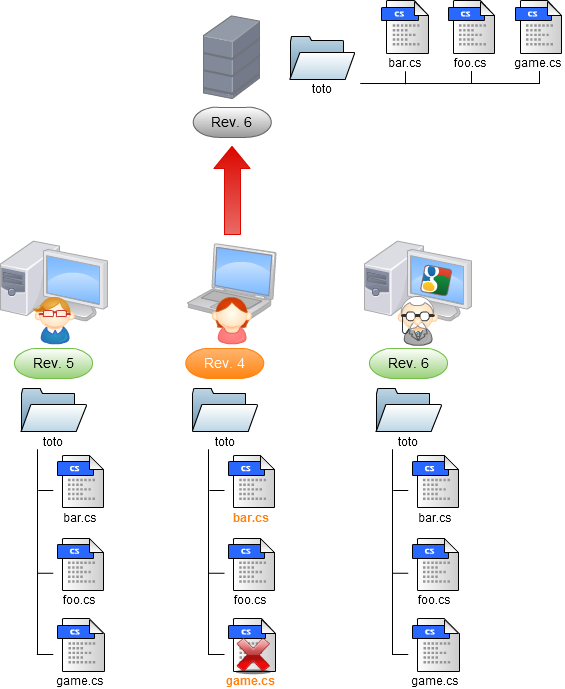
\includegraphics[scale=0.3]{images/8-Commit3.png}
  \end{center}
	% La fille essaie de commit comme une bourrine. Erreur ! elle a pas
	% update, le serveur la bloque et lui dit qu’elle n’est pas à jour.
\end{frame}

\begin{frame}
  \texttt{update}
  \begin{center}
    \vspace{-12pt}
    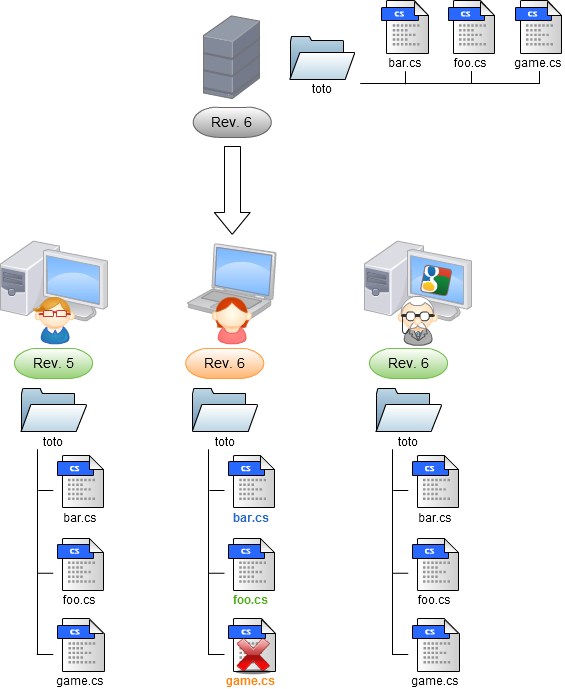
\includegraphics[scale=0.3]{images/9-Update_merge.png}
  \end{center}
	% Donc elle commence par update, ça l’amène à la révision 6, tout en
	% gardant ses modifications locales.
	% Et SVN merge bar.cs, ça fusionne les modifications récentes enregistrées
	% par le dépôt ainsi que ses modifications locales et si les deux sont
	% compatibles, il arrive à le faire proprement.
\end{frame}

\begin{frame}
  \texttt{commit}
  \begin{center}
    \vspace{-12pt}
    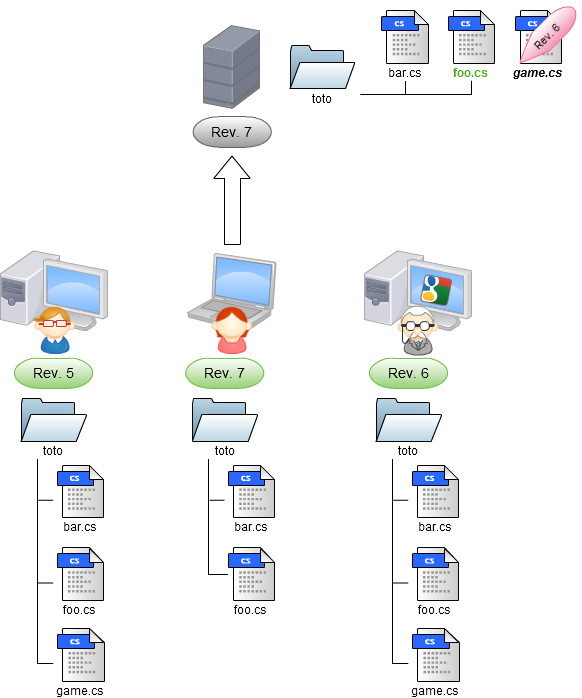
\includegraphics[scale=0.3]{images/10-Commit4.png}
  \end{center}
	% Elle commit tout son basard ! game.cs est conservé sur le dépôt par ce
	% qu’il reste une trace de tous les fichiers même supprimé, mais il est
	% n’est pas présent dans la révision actuelle.
\end{frame}

\begin{frame}
  \texttt{update}
  \begin{center}
    \vspace{-12pt}
    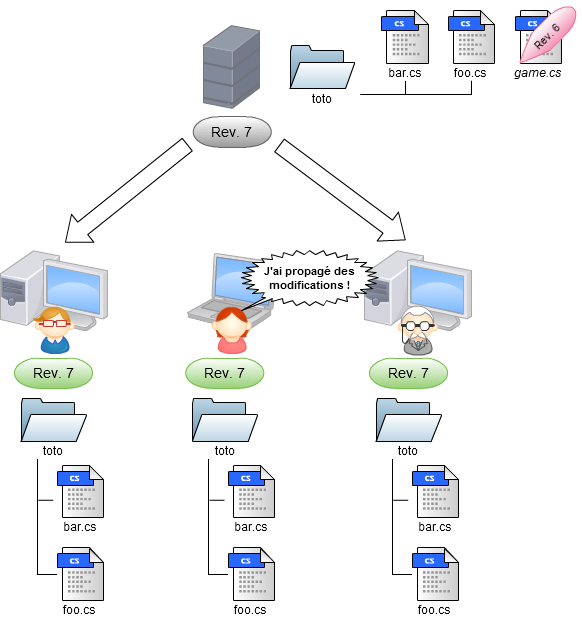
\includegraphics[scale=0.3]{images/11-Update.png}
  \end{center}
	% Elle est toute contente (imiter la fille « wahoo j’ai bien travaillé ! »),
	% et dis aux autres d’update. Ils le font et n’ont plus de game.cs
\end{frame}

\begin{frame}
  \begin{center}
    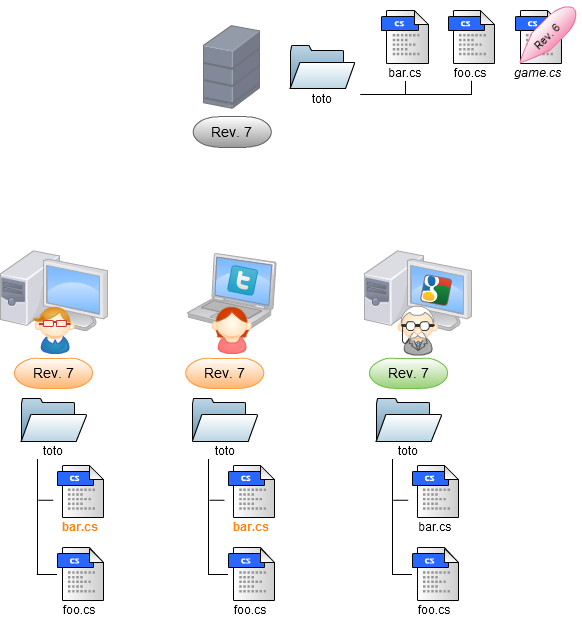
\includegraphics[scale=0.3]{images/12-Work.png}
  \end{center}
	% De retour au travail : elle change un truc dans bar.cs et va sur tweeter.
	% Mais ce qu’elle a commit ne compilait pas. Il faut toujours commit un
	% truc qui marche !
	% Le jeune résout le souçit.
\end{frame}

\begin{frame}
  \texttt{commit}
  \begin{center}
    \vspace{-12pt}
    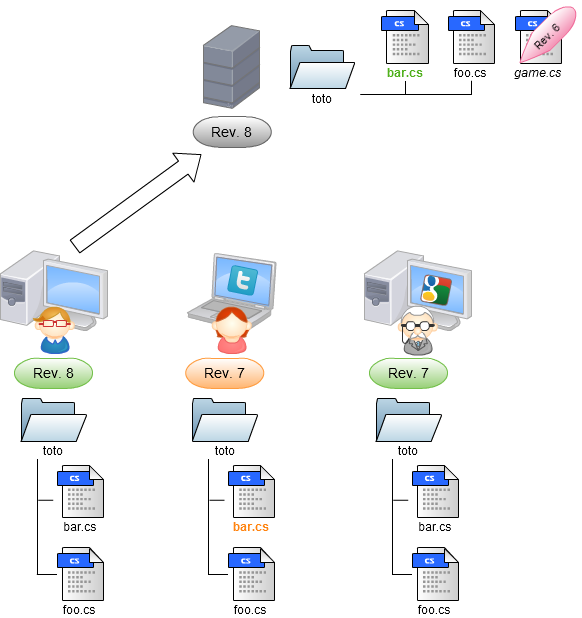
\includegraphics[scale=0.3]{images/13-Commit4.png}
  \end{center}
	% Il commit son fix des conneries de la fille.
\end{frame}

\begin{frame}
  \texttt{update}
  \begin{center}
    \vspace{-12pt}
    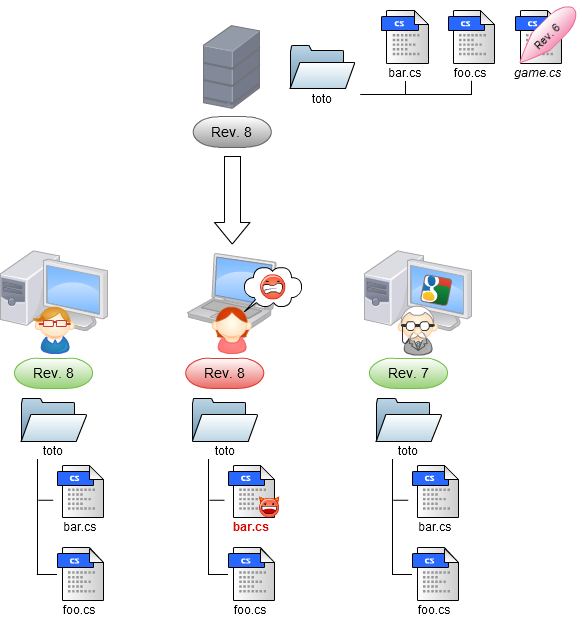
\includegraphics[scale=0.3]{images/14-Conflict.png}
  \end{center}
	% La fille veut commiter les changements qu’elle avait fait avant sa
	% session tweeter sur bar.cs, mais a retenu la leçon et update avant. Mais
	% là il y a conflit sur bar.cs, c’est à dire que SVN n’a pas réussie à
	% fusionner leur deux travail, probablement par ce que le jeune et la
	% fille vienne de modifier les même lignes de code.
\end{frame}

\begin{frame}
  \texttt{resolve}\\
  \texttt{commit}
  \begin{center}
    \vspace{-24pt}
    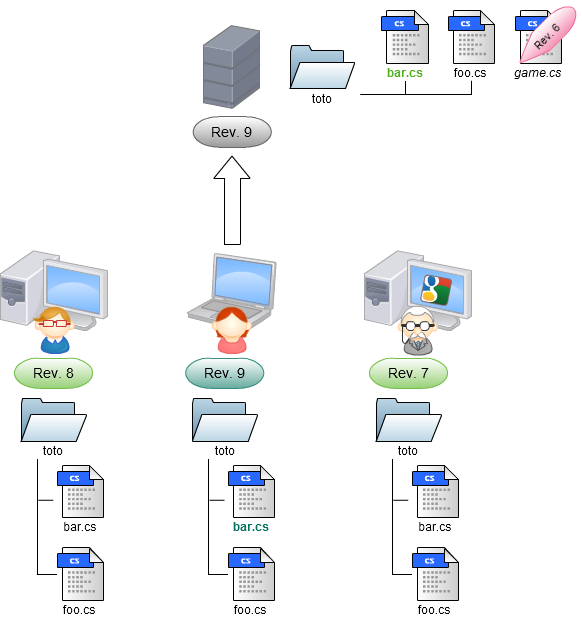
\includegraphics[scale=0.3]{images/15-Resolved.png}
  \end{center}
	% Elle résout le contenu d’une façon ou d’une autre : mon truc c’est de la
	% merde, je vais prendre la version qui est sur le dépôt, mon truc c’est
	% le meilleur, les autres c’est des gros cons ou alors essayer de comparer
	% les deux versions et de fusionner à la main (très peu probable pour
	% elle).
	% Elle indique le conflit comme «resolved» et envoie le résultat.
\end{frame}

\begin{frame}
  \begin{center}
    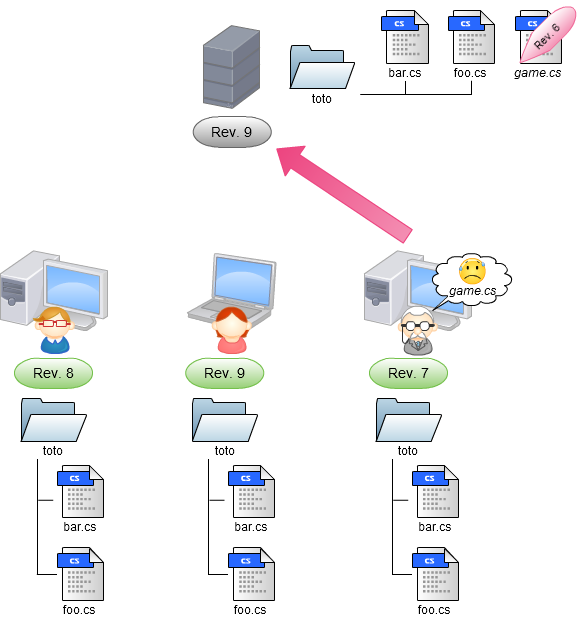
\includegraphics[scale=0.3]{images/16-Back1.png}
  \end{center}
	% Le vieux a fini sa recherche et veut travailler sur game.cs mais il se
	% rend compte qu’il a été supprimé. Mais SVN c’est trop bien, il va
	% pouvoir aller récupérer le fichier !
\end{frame}

% TODO : peut être ajouter un exemple de revert ?

\subsection{Commandes usuelles}

\begin{frame}{Subversion survival package}
  \begin{block}{Checkout -- co}
    Récupération du contenu d'un dépôt (désigné par une URL) à une version donnée.
  \end{block}
  \begin{block}{Update -- up}
    Mise à jour du contenu d'un dossier/fichier sous versionnement par rapport à la référence.
  \end{block}
  \begin{block}{Commit -- ci}
    Enregistrement des modifications effectuées sur le serveur.
  \end{block}
  \begin{block}{Add / delete}
    Activer et désactiver le versionnement sur un dossier/fichier.
  \end{block}
  % Les quatres commandes pour survivre. On peut tout faire avec.
  % Checkout : bien pour récupérer le dépôt au départ mais aussi quand vous en
  % avez marre, que plus rien de marche, vous supprimez tout et vous re-checkout
  % le dépôt en entier.
  % Update : récupère les mise à jour.
  % Commit : envoyer ses modifications.
  % Add / delete : ajouter et supprimer des fichiers au dépôt. Il faut commit
  % après et vos fichiers seront ajouter au versionnement ou supprimé. Mais
  % SVN gardent les fichier supprimés, il ne seront juste pas mis à jour.
\end{frame}



\subsection{Environnement de travail}
\begin{frame}
  \begin{center}
    
\includegraphics[scale=0.35]{images/logo_tortoise}
  \end{center}
  \begin{alertblock}{TortoiseSVN}
    \begin{itemize}
      \item S'intégre parfaitement à Windows,
      \item Ajout d'action sur les fichiers et dossiers (clic droit),
      \item Modification visuelle pour les dossiers et fichiers sous versionnement.
    \end{itemize}
	  % Permet d’avoir une interface complètement intégrée et simple
	  % d’utilisation, avec de gros boutons.
    \end{alertblock}
\end{frame}

\begin{frame}
  \begin{figure}
    \begin{center}
      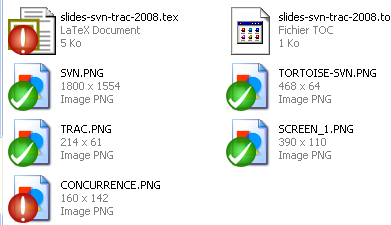
\includegraphics[scale=0.7]{images/dirView}
	  % Rouge : fichier modifié localement, les modif n’ont pas été envoyées
	  % sur le dépôt. Vert : fichier à jour avec le dépôt. Rien : pas
	  % versionné, le fichier et ses modifications ne sont pas envoyées sur le
	  % serveur.
    \end{center}
  \end{figure}
\end{frame}
\begin{frame}
  \begin{figure}
    \begin{center}
      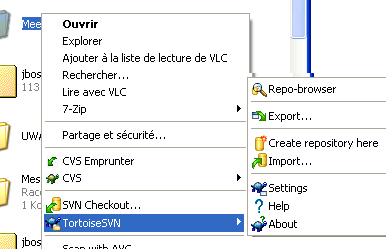
\includegraphics[scale=0.7]{images/actions}
	  % Menu intégré à l’explorateur, avec toutes les fonctions qu’on a
	  % décrite accessibles facilement.
    \end{center}
  \end{figure}
\end{frame}

\subsection{Bonnes pratiques}
\begin{frame}
  \begin{alertblock}{Update}
    Effectuer des updates régulièrement.
  \end{alertblock}
  % Update très régulièrement et *toujours* avant de commit.
  \begin{alertblock}{Commit}
    Commiter \textbf{régulièrement} du code qui \textbf{compile}.
  \end{alertblock}
  % Quand on commit, on fait toujours
  % attention que notre merde fonctionne, sinon vous allez être détesté par
  % votre groupe.
  \begin{alertblock}{Add}
    Ne pas mettre sous versionnement~:
    \begin{itemize}
    \item Les fichiers compilés par votre code (.exe, .o, .out, \ldots),
    \item Les fichiers propres à votre environnement de travail,
    \item Les fichiers systèmes (Thumbs.db, \ldots),
    \item Des fichiers inutiles (SVN n'est pas un système de partage de fichiers).
    \end{itemize}
	% On ajoute pas des fichiers compilé, on ajoute pas une vidéo d’intro de
	% 300Mo sinon à chaque fois que quelqu’un va vouloir checkout, il va se
	% tapper la vidéo à télécharger et c’est pas cool.
  \end{alertblock}
\end{frame}

\subsection{Où trouver un dépôt~?}
\begin{frame}
  \begin{exampleblock}{Les dépôts gratuits}
    \begin{itemize}
    \item GoogleCode
    \item SourceForge
    \item Assembla
    \end{itemize}
	% Vous pouvez trouver des dépôt gratuit chez ces fournisseurs. Ils
	% fournissent tous de bonnes interfaces. Googlecode et Sourceforge sont
	% les mieux. Fournis un wiki qui permet de libérer ses pulsions
	% créatrices, le système de ticket, vous créer un ticket pour chaque bug
	% ou feature manquante et vous pouvez changer son statut et la personne
	% qui doit s’en charger avec des commentaires, ou encore voir le code en
	% ligne.
  \end{exampleblock}
\end{frame}
